\chapter{El control del dron en la simulación}
\label{cap:control-sim}

\begin{enpocas}
Cómo quedaron implementados, en la simulación, el PD en cascada y el super-twisting adaptativo con sus
tres discretizaciones, con qué parámetros, y qué resultados dieron con el Tarot y con viento.
\end{enpocas}

\section{Modelo}

Cuerpo rígido con posición $p\in\mathbb{R}^3$ (marco del mundo), orientación $R\in SO(3)$ y
velocidad angular $\omega$ (marco del cuerpo):
\begin{equation}
m\ddot p = -mg\,e_3 + T R e_3 + d(t),\qquad
J\dot\omega = -\omega\times J\omega + \tau,\qquad \dot R = R\,\hat\omega,
\end{equation}
con $T$ y $\tau$ producidos por los motores a través del mezclador y $d(t)$ la perturbación
(viento). Gazebo integra el modelo completo (incluidos el retardo de los motores, el arrastre de
los rotores y el contacto con el suelo); el controlador usa los mismos $m$, $J$, $k_f$ y $k_m$.

\section{Controlador PD en cascada (línea base)}

\cod{controlador_pd.py} corre cada $T_s$ (5~ms por omisión) de tiempo simulado y manda las
velocidades de rotor con retenedor de orden cero.

\textbf{Lazo externo.} Con $e_p = p_d - p$ y $e_v = v_d - v$:
\begin{equation}
F = m\,(a + g\,e_3),\qquad a = a_d + K_p e_p + K_d e_v,\qquad T = F\cdot R e_3,
\end{equation}
con $K_p = \operatorname{diag}(4,4,6)$ y $K_d = \operatorname{diag}(3,3,4)$.

\textbf{Actitud deseada.} A partir de la dirección de $F$ y la guiñada deseada $\psi_d$:
\begin{equation}
b_3 = \frac{F}{\|F\|},\quad b_{1c} = (\cos\psi_d,\sin\psi_d,0),\quad
b_2 = \frac{b_3\times b_{1c}}{\|b_3\times b_{1c}\|},\quad R_d = [\,b_2\times b_3,\ b_2,\ b_3\,].
\end{equation}

\textbf{Lazo interno} (PD sobre SO(3)):
\begin{equation}
e_R = \tfrac12\big(R_d^\top R - R^\top R_d\big)^\vee,\qquad
\tau = -K_R e_R - K_\omega\,\omega + \omega\times J\omega .
\end{equation}

\section{Super-twisting adaptativo (STA)}

\cod{controlador_sta.py} reemplaza la aceleración del lazo externo. Por eje:
\begin{equation}
s = e_v + \lambda e_p,\qquad a = a_d + \lambda e_v - u
\quad\Rightarrow\quad \dot s = u + d(t),
\end{equation}
y $u$ es el super-twisting con ganancia adaptativa (Shtessel, Taleb y Plestan, 2012):
\begin{align}
u &= -k_1 |s|^{1/2}\sgn(s) + \nu, & \dot\nu &= -k_2\sgn(s),\\
\dot k_1 &= \begin{cases} w_1\sqrt{\gamma_1/2}\;\sgn(|s|-\mu) & k_1 > k_{1,min}\\ \eta & \text{en otro caso}\end{cases},
& k_2 &= 2\varepsilon k_1 .
\end{align}

\subsection{Discretizaciones}
\label{sec:discretizaciones}

Con periodo $T_s$ y $a_k = s_k + T_s\nu_k$, \cod{sta.py} implementa:

\begin{description}
  \item[Explícita] $u_k = -k_1|s_k|^{1/2}\sgn(s_k) + \nu_k$,\quad $\nu_{k+1} = \nu_k - T_s k_2\sgn(s_k)$.
  \item[Semi-implícita] el término discontinuo se evalúa en el paso siguiente y $|s|^{1/2}$ en el actual:
        $\tilde s + (T_s k_1|s_k|^{1/2} + T_s^2 k_2)\,\xi = a_k$, con $\xi\in\Sgn(\tilde s)$.
  \item[Implícita] (Brogliato, Polyakov y Efimov, 2020):
  \begin{equation}
  \tilde s + T_s k_1|\tilde s|^{1/2}\xi + T_s^2 k_2\,\xi = a_k,\qquad \xi\in\Sgn(\tilde s),
  \end{equation}
  cuya solución única es
  \begin{equation}
  \begin{cases}
  \tilde s = 0,\quad \xi = a_k/(T_s^2k_2) & \text{si } |a_k|\le T_s^2k_2,\\[2pt]
  \tilde s = \sgn(a_k)\,w^2,\quad w = \dfrac{-T_sk_1+\sqrt{T_s^2k_1^2+4(|a_k|-T_s^2k_2)}}{2} & \text{en otro caso.}
  \end{cases}
  \end{equation}
\end{description}
En los dos esquemas implícitos $\tilde s$ es la predicción nominal de $s_{k+1}$, $\nu_{k+1} = \nu_k
- T_s k_2\xi$ y $u_k = (\tilde s - s_k)/T_s$. El código de la solución implícita:

\begin{lstlisting}[style=py]
@staticmethod
def resolver_implicito(a, b, c):
    """Solución única de  x + b |x|^(1/2) xi + c xi = a,  xi en Sgn(x),  b, c > 0."""
    abs_a = np.abs(a)
    dentro = abs_a <= c
    w = (-b + np.sqrt(b**2 + 4.0 * np.maximum(abs_a - c, 0.0))) / 2.0
    x = np.where(dentro, 0.0, np.sign(a) * w**2)
    xi = np.where(dentro, a / np.where(dentro, c, 1.0), np.sign(a))
    return x, xi
\end{lstlisting}

\subsection{Parámetros}

En \cod{config/parametros.yaml}, sección \cod{controlador_sta}: $\lambda = (1.5, 1.5, 2.0)$,
$k_{1,0} = 1$, $\varepsilon = 1$, $w_1 = 2$, $\gamma_1 = 1$, $k_{1,min} = 0.5$, $\eta = 0.1$. Los que
dependen del vehículo van en su YAML: para el Tarot $\mu = (0.3, 0.3, 0.03)$ y $k_{1,max} = 3$.
El esquema se elige al lanzar:
\begin{lstlisting}[style=bash]
ros2 launch cuadrirotor_sim simulacion.launch.py vehiculo:=tarot650 mundo:=bosque \
    controlador:=sta esquema:=implicito mision:=orbita viento:=true csv:=$HOME/corrida.csv
\end{lstlisting}

\section{Resultados}

La misión \cod{orbita} despega a 3~m, se traslada y describe una órbita de radio 4~m alrededor del
foco $(8,5)$ con la cámara apuntando a él, con viento desde
$t = 15$~s. Las métricas las calcula \cod{scripts/metricas.py}.

\begin{figure}[H]
\centering
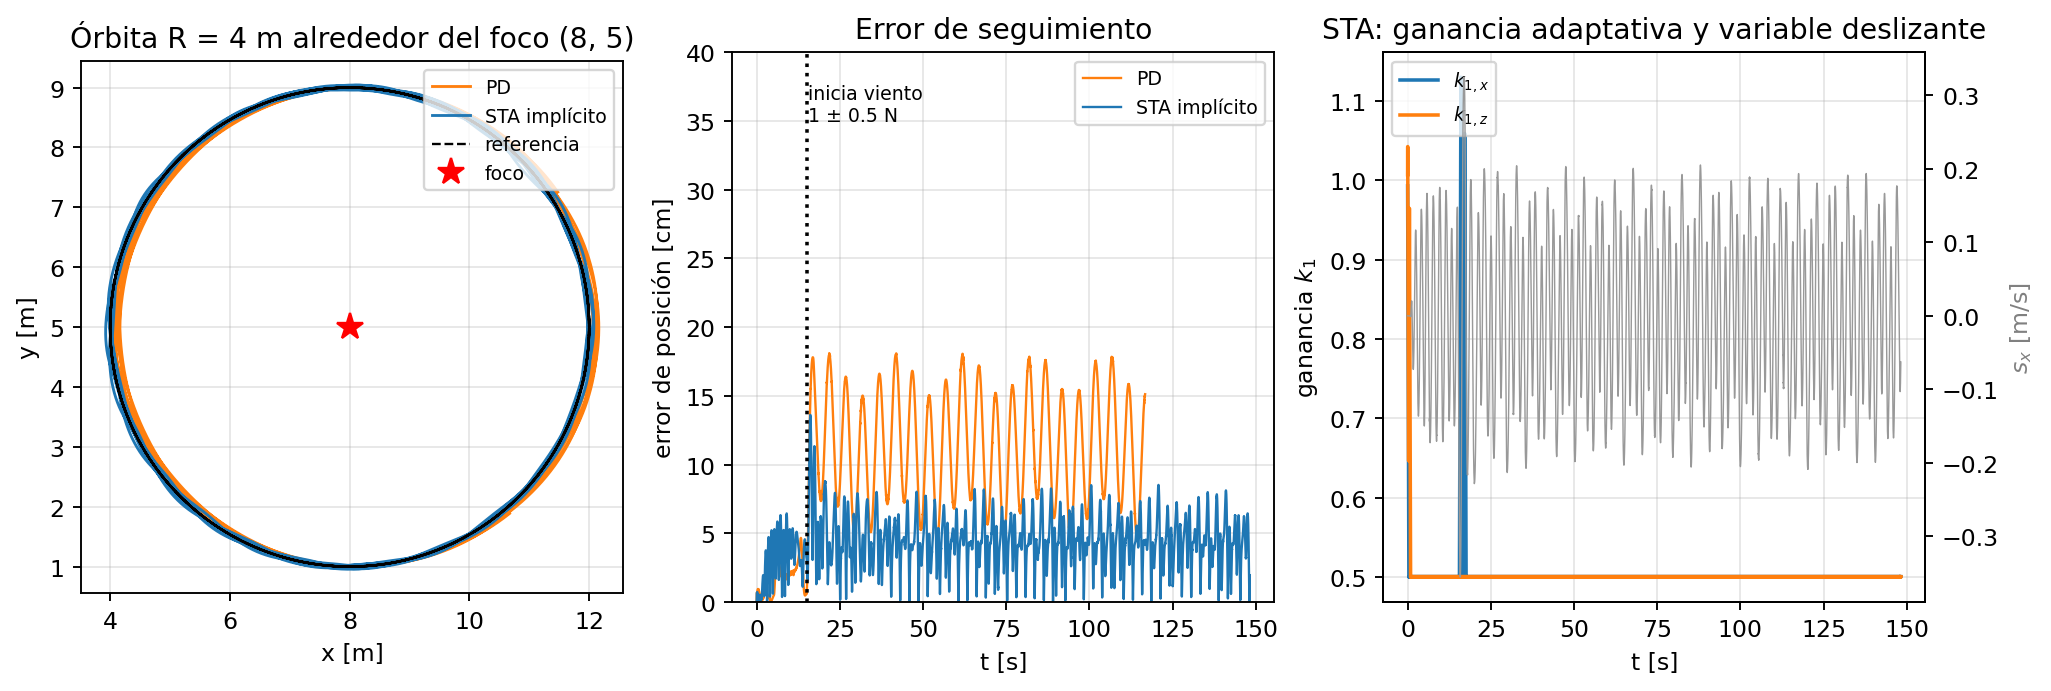
\includegraphics[width=\textwidth]{orbita_pd_sta.png}
\caption{Tarot 650 en el mundo \cod{bosque}, órbita con viento de $1\pm0.5$~N (corridas del 23 de
octubre). El STA implícito reduce el error RMS con viento de 11.9~cm (PD) a 4.8~cm. La ganancia
$k_1$ baja hasta $k_{1,min}$: el umbral $\mu$ del Tarot queda por encima del ciclo límite.}
\label{fig:orbita}
\end{figure}

\begin{table}[H]
\centering\small
\begin{tabular}{llccc}
\toprule
\textbf{Vehículo} & \textbf{Controlador} & \textbf{RMS sin viento} & \textbf{RMS con viento} & \textbf{Máx. con viento} \\ \midrule
cuadrirrotor & PD en cascada & --- & 17.7 cm & 28.5 cm \\
cuadrirrotor & STA explícito & --- & 2.4 cm & 4.7 cm \\
cuadrirrotor & STA semi-implícito & --- & 2.1 cm & 4.0 cm \\
cuadrirrotor & STA implícito & --- & 2.1 cm & 4.3 cm \\
Tarot 650 & PD en cascada & 2.8 cm & 11.9 cm & 18.1 cm \\
Tarot 650 & STA implícito & 3.3 cm & 4.8 cm & 8.5 cm \\
Tarot 650 & ArduCopter 4.7.2 & --- & 13.7 cm & --- \\
\bottomrule
\end{tabular}
\caption{Error de seguimiento en la órbita ($T_s = 5$~ms). Las filas del cuadrirrotor y la de
ArduPilot son del 21--22 de octubre; las del Tarot con PD y STA, de las corridas de la
figura~\ref{fig:orbita}.}
\end{table}

\subsection{Observaciones}
\label{sec:observaciones}

\begin{enumerate}
  \item Con perturbación, el esquema implícito de las ec.~(9)--(12) deja una banda
        $|s|\approx T_s|d|$, \textbf{independiente de la ganancia} (insensible a la
        sobreestimación), pero no proporcional a $T_s^2k_2$ como plantea la hipótesis: la predicción
        nominal supone $d=0$. Con \cod{estimar_perturbacion: true} (estimación $\hat d$ del paso
        anterior; Acary, Brogliato y Orlov, 2012) la banda baja a $\approx T_s^2\max|\dot d|$.
  \item En $x$, $y$ el retardo del lazo de actitud y de los motores induce un ciclo límite
        ($|s|\approx$ 0.05--0.1~m/s en el cuadrirrotor, 0.2--0.35~m/s en el Tarot). Si $\mu$ queda
        por debajo de él, la ganancia crece sin control y el lazo se inestabiliza; por eso $\mu$
        es por eje y por vehículo.
  \item La velocidad que publica Gazebo es un promedio de 10 muestras ($\approx$4.5~ms de retraso
        a 1~kHz): forma parte de la dinámica no modelada.
\end{enumerate}

\section{Agregar un controlador}

Se hereda de \cod{ControladorPD}, se sobrescribe \cod{aceleracion(ep, ev, ad)} y se registra el
ejecutable en \cod{setup.py}. Así quedó el STA:
\begin{lstlisting}[style=py]
def aceleracion(self, ep, ev, ad):
    self.s = ev + self.lam * ep
    return ad + self.lam * ev - self.sta(self.s)
\end{lstlisting}
